\documentclass{article}

\usepackage{cancel}
\usepackage{algorithm} %pseudo-code
\usepackage{algpseudocode}
\usepackage[top=1.5in, bottom=1.5in, left=1.5in, right=1.5in]{geometry}
\usepackage{amsmath,amsthm,amssymb}
\usepackage{graphicx}
\usepackage{float}
\usepackage{amsmath, amssymb, amscd}
\usepackage{alltt}
\usepackage{textcomp}
\usepackage{gensymb}
\usepackage{multicol}
\usepackage{tabularx}
\usepackage{units}
%\usepackage{mathpple}
%\usepackage{mathpazo}
\usepackage{fouriernc}
%\usepackage{euler}
\usepackage[mathscr]{euscript}

\newcommand{\N}{\mathbb{N}}
\newcommand{\Z}{\mathbb{Z}}
\newcommand{\R}{\mathbb{R}}
\newcommand{\bigo}{\mathcal{O}}
\newcommand{\G}{\mathcal{G}}
\newcommand{\V}{\mathcal{V}}
\newcommand{\E}{\mathcal{E}}
\newcommand{\K}{\mathcal{K}}
\newcommand{\T}{^\intercal}

\def\changemargin#1#2{\list{}{\rightmargin#2\leftmargin#1}\item[]}
\let\endchangemargin=\endlist 

\newcommand{\sups}[1]{\ensuremath{^{\textrm{#1}}}}
\newcommand{\subs}[1]{\ensuremath{_{\textrm{#1}}}}

\newcommand{\specialcell}[2][c]
{
  \begin{tabular}[#1]{@{}c@{}}#2\end{tabular}
}

\makeatletter
\newsavebox{\mybox}\newsavebox{\mysim}
\newcommand{\distras}[1]
{
  \savebox{\mybox}{\hbox{\kern3pt$\scriptstyle#1$\kern3pt}}%
  \savebox{\mysim}{\hbox{$\sim$}}%
  \mathbin{\overset{#1}{\kern\z@\resizebox{\wd\mybox}{\ht\mysim}{$\sim$}}}%
}
\makeatother

% aligned matrix negative signs:
\makeatletter
\renewcommand*\env@matrix[1][c]{\hskip -\arraycolsep
  \let\@ifnextchar\new@ifnextchar
  \array{*\c@MaxMatrixCols #1}}
\makeatother

%===============================================================================
% code highlighting :
\usepackage{listings}

% define custom colors :
\usepackage{color}
\definecolor{bg}{rgb}{0.96,0.96,0.85}
\definecolor{deepblue}{rgb}{0,0,0.5}
\definecolor{deepred}{rgb}{0.6,0,0}
\definecolor{deepgreen}{rgb}{0,0.5,0}

\usepackage{xcolor}
\renewcommand{\lstlistlistingname}{Code Listings}
\renewcommand{\lstlistingname}{Code Listing}
\definecolor{gray}{gray}{0.5}
\colorlet{commentcolour}{green!50!black}

\colorlet{stringcolour}{red!60!black}
\colorlet{keywordcolour}{magenta!90!black}
\colorlet{exceptioncolour}{yellow!50!red}
\colorlet{commandcolour}{blue!60!black}
\colorlet{numpycolour}{blue!60!green}
\colorlet{literatecolour}{magenta!90!black}
\colorlet{promptcolour}{green!50!black}
\colorlet{specmethodcolour}{violet}
\colorlet{indendifiercolour}{green!70!white}

\newcommand{\framemargin}{5ex}

\newcommand{\literatecolour}{\textcolor{literatecolour}}

\newcommand\Small{\fontsize{1.00}{5.0}\selectfont}

\newcommand\pythonstyle{\lstset{
%keepspaces=true,
language=python,
showtabs=true,
tab=,
tabsize=2,
basicstyle=\ttfamily\Small,%\setstretch{.5},
stringstyle=\color{stringcolour},
showstringspaces=false,
alsoletter={1234567890},
otherkeywords={\ , \}, \{, \%, \&, \|},
keywordstyle=\color{keywordcolour}\bfseries,
emph={and,break,class,continue,def,yield,del,elif ,else,%
except,exec,finally,for,from,global,if,import,in,%
lambda,not,or,pass,print,raise,return,try,while,assert},
emphstyle=\color{blue}\bfseries,
emph={[2]True, False, None},
emphstyle=[2]\color{keywordcolour},
emph={[3]object,type,isinstance,copy,deepcopy,zip,enumerate,reversed,list,len,dict,tuple,xrange,append,execfile,real,imag,reduce,str,repr},
emphstyle=[3]\color{commandcolour},
emph={Exception,NameError,IndexError,SyntaxError,TypeError,ValueError,OverflowError,ZeroDivisionError},
emphstyle=\color{exceptioncolour}\bfseries,
%upquote=true,
morestring=[s]{"""}{"""},
morestring=[s]{'''}{'''},
commentstyle=\color{commentcolour}\slshape,
%emph={[4]1, 2, 3, 4, 5, 6, 7, 8, 9, 0},
emph={[4]ode, fsolve, sqrt, exp, sin, cos, arccos, pi,  array, norm, solve, dot, arange, , isscalar, max, sum, flatten, shape, reshape, find, any, all, abs, linspace, legend, quad, polyval,polyfit, hstack, concatenate,vstack,column_stack,empty,zeros,ones,rand,vander,grid,pcolor,eig,eigs,eigvals,svd,qr,tan,det,logspace,roll,min,mean,cumsum,cumprod,diff,vectorize,lstsq,cla,eye,xlabel,ylabel,squeeze,plot,median,std,hist},
emphstyle=[4]\color{numpycolour},
emph={[5]__init__,__add__,__mul__,__div__,__sub__,__call__,__getitem__,__setitem__,__eq__,__ne__,__nonzero__,__rmul__,__radd__,__repr__,__str__,__get__,__truediv__,__pow__,__name__,__future__,__all__},
emphstyle=[5]\color{specmethodcolour},
emph={[6]assert,range,yield},
emphstyle=[6]\color{keywordcolour}\bfseries,
% emph={[7]self},
% emphstyle=[7]\bfseries,
literate=*%
{:}{{\literatecolour:}}{1}%
{=}{{\literatecolour=}}{1}%
{-}{{\literatecolour-}}{1}%
{+}{{\literatecolour+}}{1}%
{*}{{\literatecolour*}}{1}%
{/}{{\literatecolour/}}{1}%
{!}{{\literatecolour!}}{1}%
%{(}{{\literatecolour(}}{1}%
%{)}{{\literatecolour)}}{1}%
{[}{{\literatecolour[}}{1}%
{]}{{\literatecolour]}}{1}%
{<}{{\literatecolour<}}{1}%
{>}{{\literatecolour>}}{1}%
{>>>}{{\textcolor{promptcolour}{>>>}}}{1}%
,%
breaklines=true,
breakatwhitespace= true,
%xleftmargin=\framemargin,
%xrightmargin=\framemargin,
aboveskip=1ex,
frame=trbl,
%frameround=tttt,
rulecolor=\color{black!40},
%framexleftmargin=\framemargin,
%framextopmargin=.1ex,
%framexbottommargin=.1ex,
%framexrightmargin=\framemargin,
%framexleftmargin=1mm, framextopmargin=1mm, frame=shadowbox, rulesepcolor=\color{blue},#1
%frame=tb,
backgroundcolor=\color{yellow!10}
}}

\newcommand\Rstyle{\lstset{
%keepspaces=true,
language=R,
showtabs=true,
tab=,
tabsize=2,
basicstyle=\ttfamily\Small,%\setstretch{.5},
stringstyle=\color{stringcolour},
showstringspaces=false,
alsoletter={1234567890},
otherkeywords={\ , \}, \{, \%, \&, \|},
keywordstyle=\color{keywordcolour}\bfseries,
emph={and,break,class,continue,def,yield,del,elif ,else,%
except,exec,finally,for,from,global,if,import,in,%
lambda,not,or,pass,print,raise,return,try,while,assert},
emphstyle=\color{blue}\bfseries,
emph={[2]True, False, None},
emphstyle=[2]\color{keywordcolour},
emph={[3]object,type,isinstance,copy,deepcopy,zip,enumerate,reversed,list,len,dict,tuple,xrange,append,execfile,real,imag,reduce,str,repr},
emphstyle=[3]\color{commandcolour},
emph={Exception,NameError,IndexError,SyntaxError,TypeError,ValueError,OverflowError,ZeroDivisionError},
emphstyle=\color{exceptioncolour}\bfseries,
%upquote=true,
morestring=[s]{"""}{"""},
morestring=[s]{'''}{'''},
commentstyle=\color{commentcolour}\slshape,
%emph={[4]1, 2, 3, 4, 5, 6, 7, 8, 9, 0},
emph={[4]ode, fsolve, sqrt, exp, sin, cos, arccos, pi,  array, norm, solve, dot, arange, , isscalar, max, sum, flatten, shape, reshape, find, any, all, abs, linspace, legend, quad, polyval,polyfit, hstack, concatenate,vstack,column_stack,empty,zeros,ones,rand,vander,grid,pcolor,eig,eigs,eigvals,svd,qr,tan,det,logspace,roll,min,mean,cumsum,cumprod,diff,vectorize,lstsq,cla,eye,xlabel,ylabel,squeeze,plot,median,std,hist},
emphstyle=[4]\color{numpycolour},
emph={[5]__init__,__add__,__mul__,__div__,__sub__,__call__,__getitem__,__setitem__,__eq__,__ne__,__nonzero__,__rmul__,__radd__,__repr__,__str__,__get__,__truediv__,__pow__,__name__,__future__,__all__},
emphstyle=[5]\color{specmethodcolour},
emph={[6]assert,range,yield},
emphstyle=[6]\color{keywordcolour}\bfseries,
% emph={[7]self},
% emphstyle=[7]\bfseries,
literate=*%
{:}{{\literatecolour:}}{1}%
{=}{{\literatecolour=}}{1}%
{-}{{\literatecolour-}}{1}%
{+}{{\literatecolour+}}{1}%
{*}{{\literatecolour*}}{1}%
{/}{{\literatecolour/}}{1}%
{!}{{\literatecolour!}}{1}%
%{(}{{\literatecolour(}}{1}%
%{)}{{\literatecolour)}}{1}%
{[}{{\literatecolour[}}{1}%
{]}{{\literatecolour]}}{1}%
{<}{{\literatecolour<}}{1}%
{>}{{\literatecolour>}}{1}%
{>>>}{{\textcolor{promptcolour}{>>>}}}{1}%
,%
breaklines=true,
breakatwhitespace= true,
%xleftmargin=\framemargin,
%xrightmargin=\framemargin,
aboveskip=1ex,
frame=trbl,
%frameround=tttt,
rulecolor=\color{black!40},
%framexleftmargin=\framemargin,
%framextopmargin=.1ex,
%framexbottommargin=.1ex,
%framexrightmargin=\framemargin,
%framexleftmargin=1mm, framextopmargin=1mm, frame=shadowbox, rulesepcolor=\color{blue},#1
%frame=tb,
backgroundcolor=\color{yellow!10}
}}

% Python environment
\lstnewenvironment{python}[1][]
{
  \pythonstyle
  \lstset{#1}
}
{}

% R environment
\lstnewenvironment{Rs}[1][]
{
  \Rstyle
  \lstset{#1}
}
{}

% Python for external files
\newcommand\pythonexternal[1]
{{
  \pythonstyle
  \lstinputlisting{#1}
}}

% Python for inline
\newcommand\pythoninline[1]
{{
  \pythonstyle
  \lstinline!#1!
}}

% answer box :
\newcommand\answer[1]
{{
  \begin{center}
    \parbox[t]{5in}{#1}
  \end{center}
}}

% end code highlighting
%===============================================================================


% border matrix with brackets :
\usepackage{etoolbox}
\let\bbordermatrix\bordermatrix
\patchcmd{\bbordermatrix}{8.75}{4.75}{}{}
\patchcmd{\bbordermatrix}{\left(}{\left[}{}{}
\patchcmd{\bbordermatrix}{\right)}{\right]}{}{}


\usepackage[backend=biber, style=authoryear, sorting=nyt]{biblatex}
\renewcommand*{\bibfont}{\normalsize}
\addbibresource{biblio.bib}

\begin{document}

\title{Determining the effect of gun laws on gun violence}
\author{Evan Cummings\\
CSCI 548 - Pattern Recognition}

\maketitle

\section{Background and significance}

Gun laws in the US are currently a major topic of discussion; US citizens want proof that newly-proposed-gun-control laws will have an effect on gun-violence.  To date, a number of different laws have been enacted such as The Firearm Owner's Protection Act of 1986, The Brady Handgun Violence Act of 1993, or The Violent Crime Control and Law Enforcement Act of 1994.  While previous studies have described the overall trend in homicide by firearms [\cite{cooper}], attempted to derive some relationship between firearm violence and firearm ownership [\cite{swedler}], or in some other way attempted to describe the causes or effects of gun-violence, this new study will evaluate the relationships between circumstances of violence at the police-department level and derive relationships between gun laws and gun violence.  For example, many people believe that prohibiting certain people from owning guns will have a decreasing effect on gun violence.  In this study we will examine the effect The Firearm Owners Protection Act -- which banned the sale of firearms to felons -- had on firearm violence from 1986 onwards.  Understanding the effect these firearm laws have on firearm violence may help indicate the effect of enacting similar laws in the future.

\section{Research description}

We will supplement the Federal Bureau of Investigation's (FBI) Uniform Crime Report (UCR) [\cite{shr}] with factors for each police-department indicating the presence or non-presence of a gun-control law in its jurisdiction for each of the years included in the data, 1975 -- 2010.  Other factors will be incorporated from the Supplemental Homicide Report (SHR) section of the UCR, such as age of the victim and offender, sex and race of offender, weapon used, circumstances surrounding the crime, population, etc.

%After some initial exploratory data analysis, clustering algorithms will be performed on the data to discover any grouping of firearm violence in the presence of gun-control laws.  Ideally, other factors such as poverty level and crime rate will be included from data provided by The US Census Bureau.

First, we will evaluate the covariance structure of the data dimensions in order to derive with certainty any overall trends contained in the data.  These trends have the potential to provide immense insight into the nature of deadly violence.  For example, this analysis may show a certain prefrence for weapon type used in familiy violence;  we could then report with some quantifiable degree of certainty the weapon most likely used in these senarios.

Next, we will examine the death-by-firearm counts for each police department jurisdiction and their relationship to gun-control-laws.  For each law, and for each jurisdiction, we can classify the region for each year as being under a certain law or not.  We can then perform linear discriminant analyses (LDA) on the data; if the data is separable by the presence of a gun-control law, we can report that the law does indeed have an affect on firarm deadly violence.


\section{Preliminary results}

\begin{figure}[H]
  \centering
    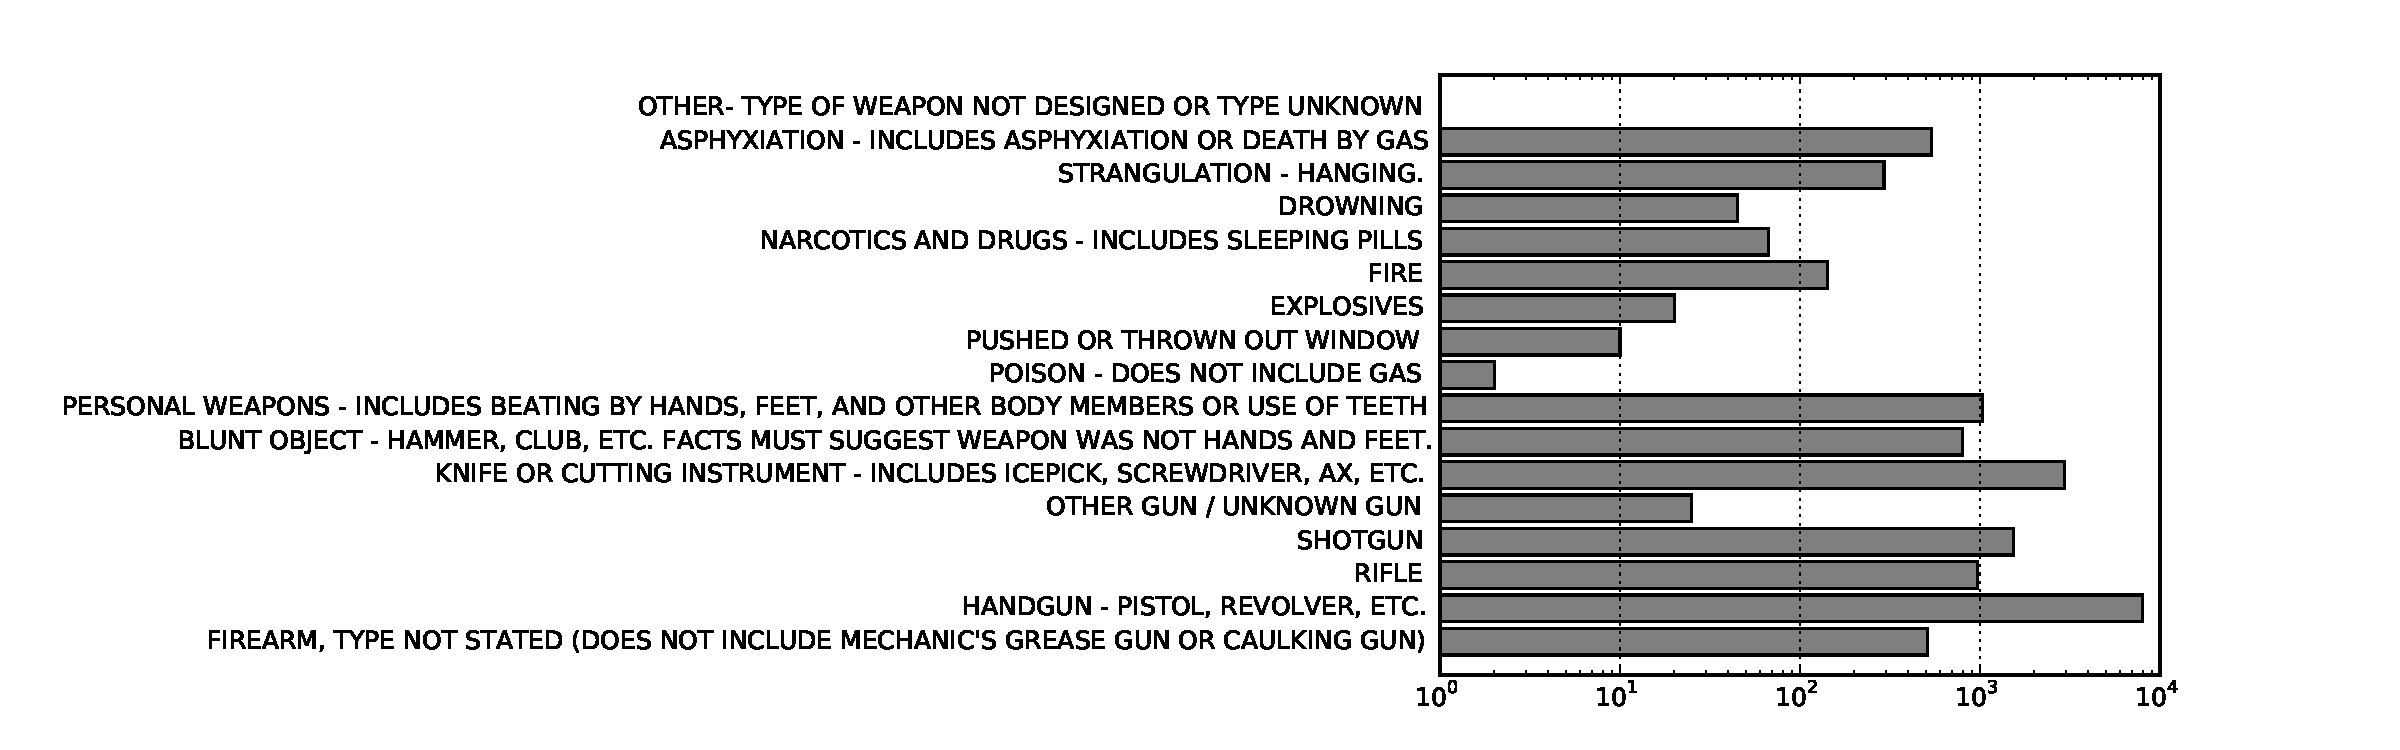
\includegraphics[width=\linewidth]{images/weaps.pdf}
    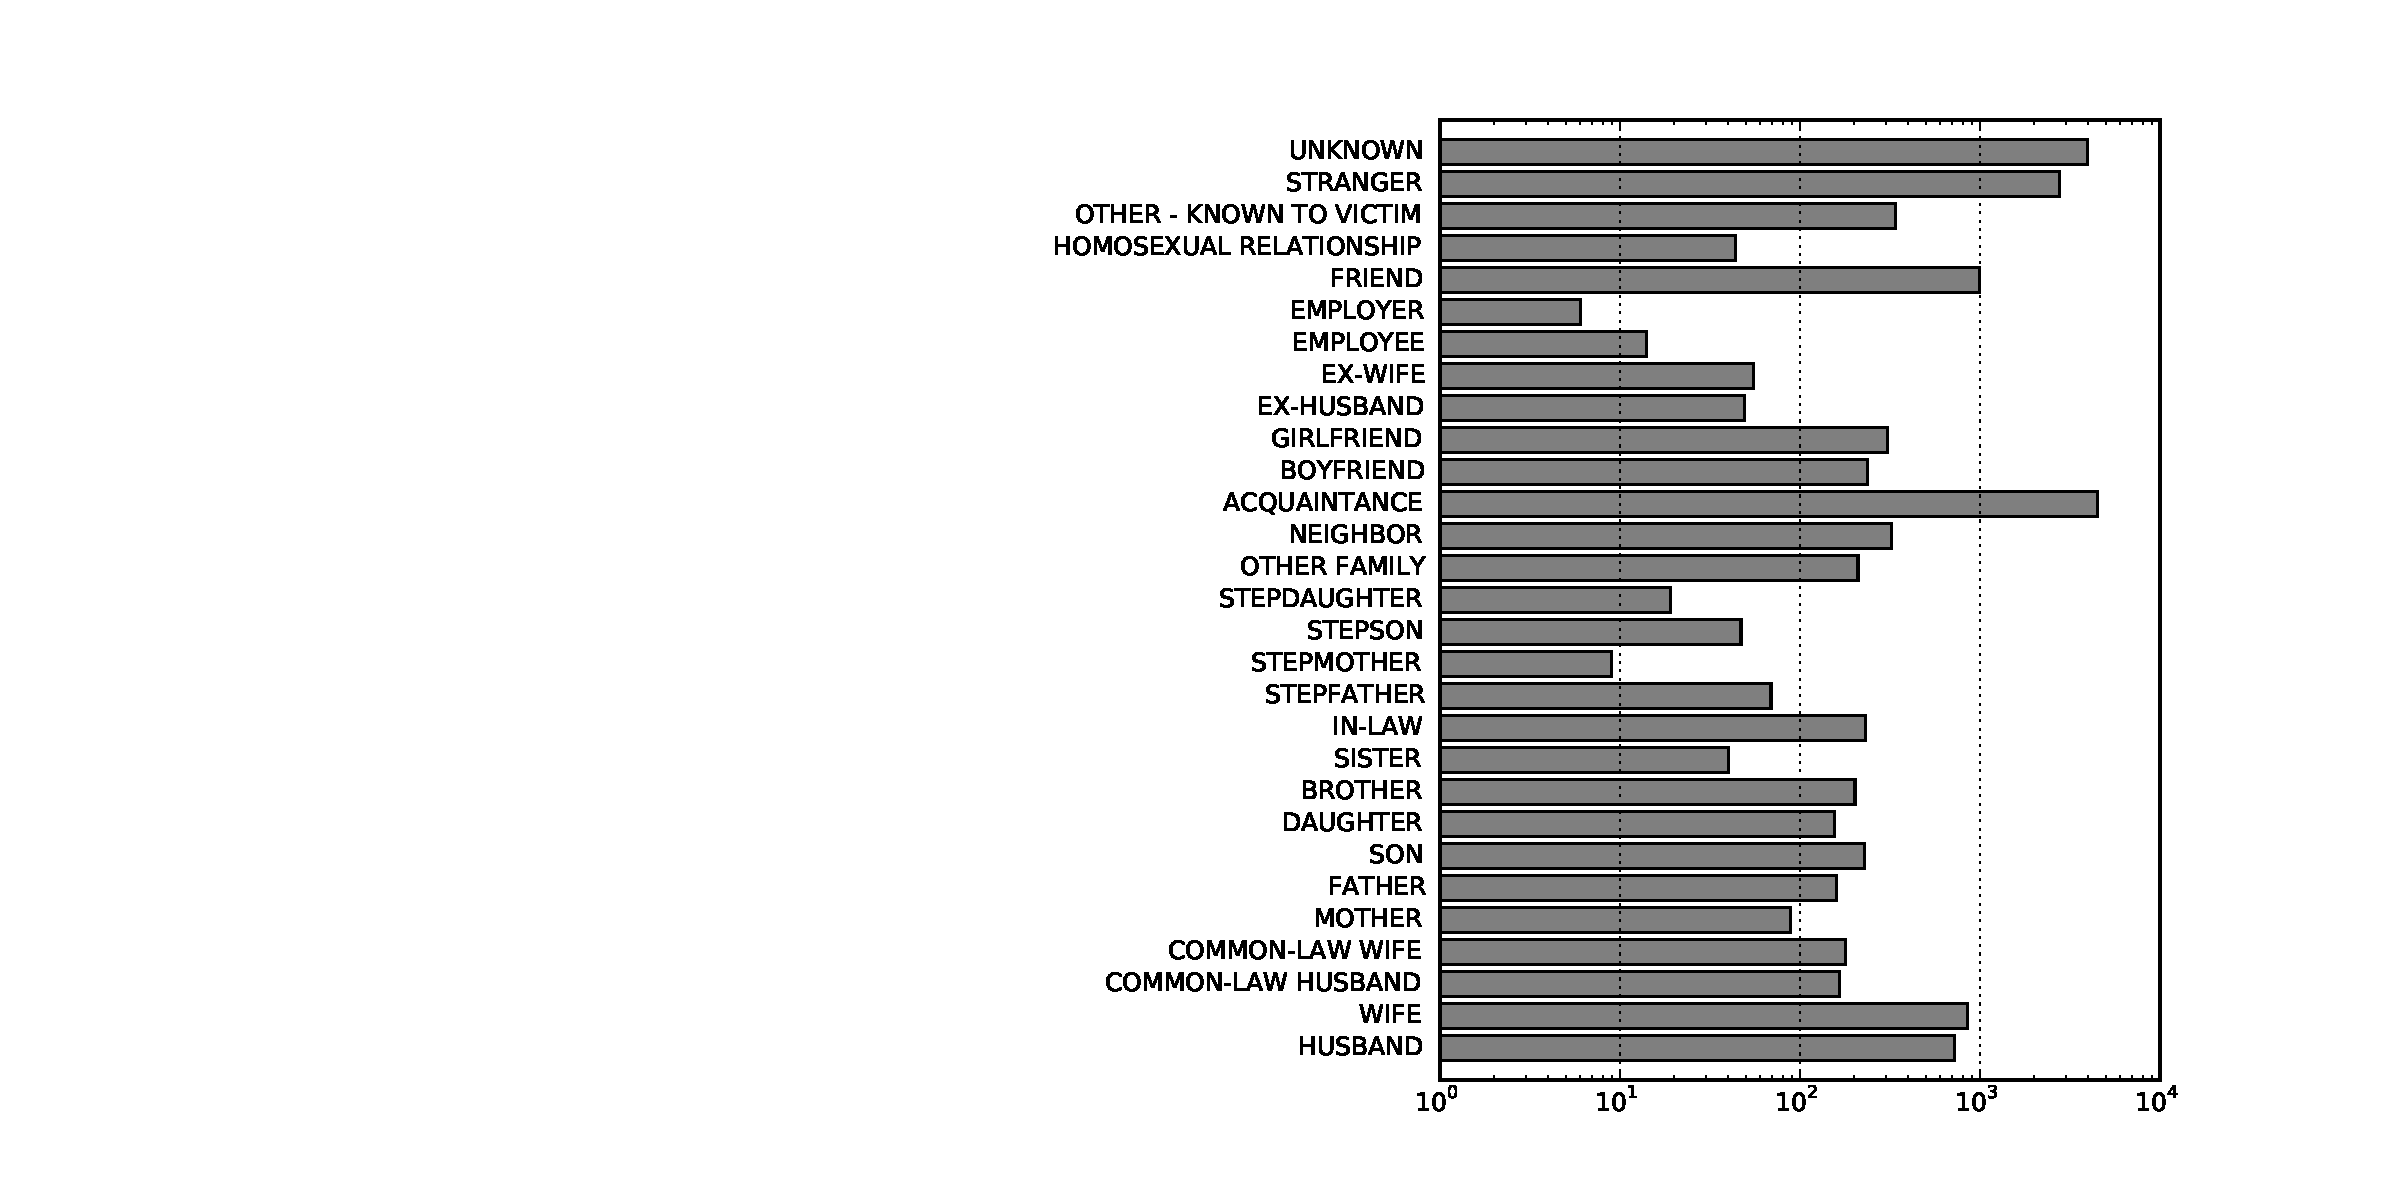
\includegraphics[width=\linewidth]{images/relationship.pdf}
    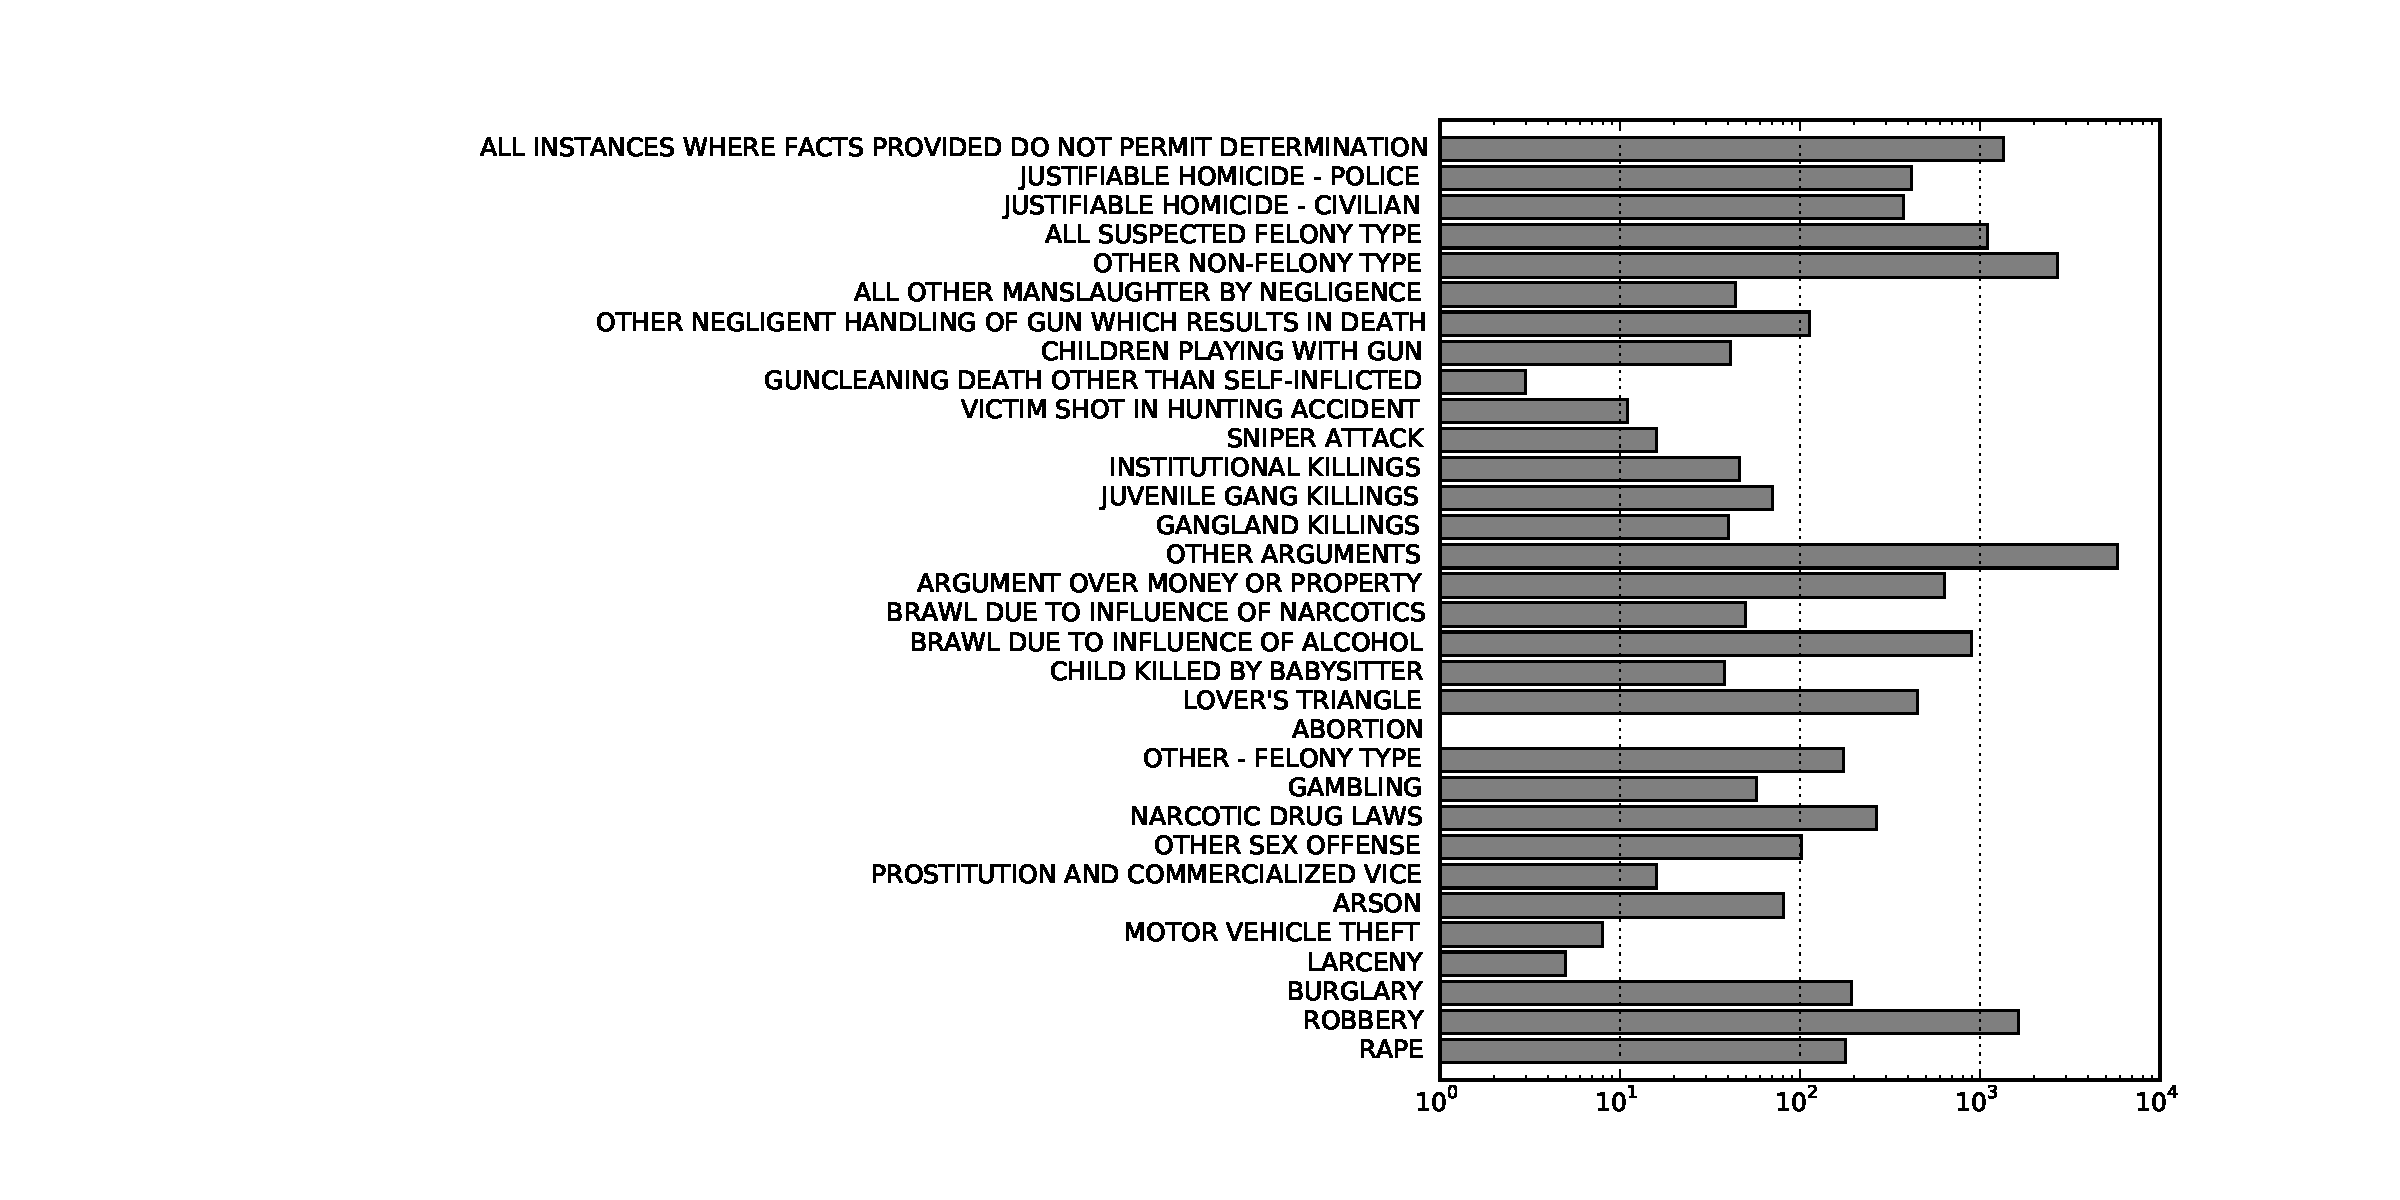
\includegraphics[width=\linewidth]{images/circumstance.pdf}
  \caption{The number of deaths in 1976 by weapon type (top), relationship of the offender to the victim (middle), and circumstances (bottom).}
\end{figure}

\begin{figure}[H]
  \centering
  \begin{minipage}[b]{0.45\linewidth}
    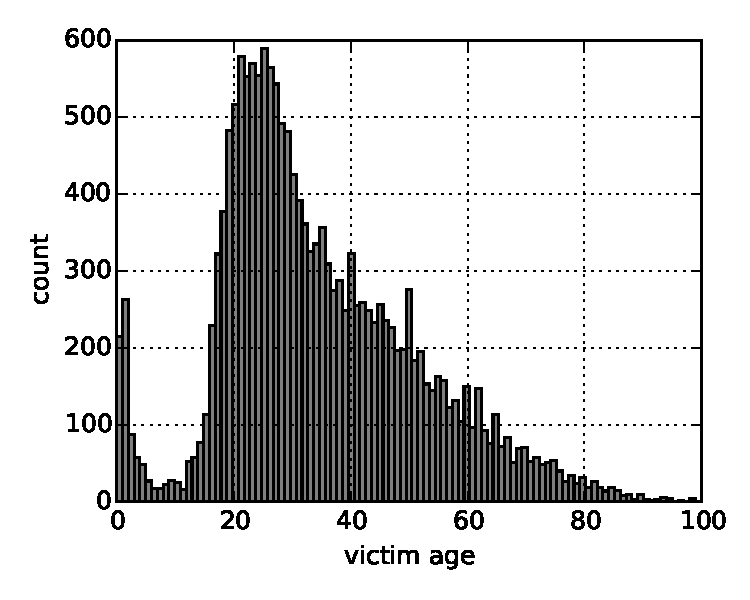
\includegraphics[width=\linewidth]{images/victim_age.pdf}
  \end{minipage}
  \quad
  \begin{minipage}[b]{0.45\linewidth}
    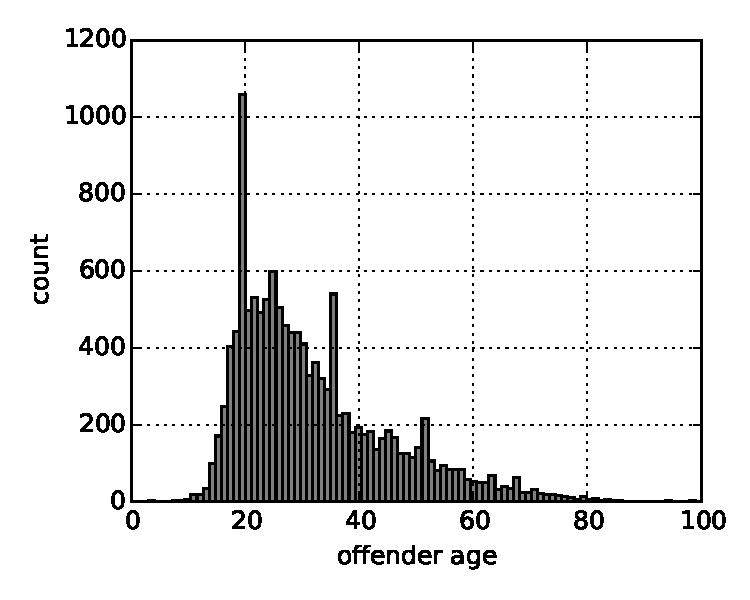
\includegraphics[width=\linewidth]{images/offender_age.pdf}
  \end{minipage}
  \caption{Histogram of victim ages (left) and offender ages (right) for 1976.}
\end{figure}

\section{Broader impacts}

If sucessful, this project may be used to evaluate crime in a region and derive an appropriate gun-control law.  It may be possible to substantially reduce gun-violent-death.  At the very least this study will provide new insight into the nature of violent death in the U.S., as well as the complicated relationship between the offenders and their victims.

\section{Project plan}

\begin{enumerate}

  \item download all the data

  \item parse the data into a uniform file format

  \item remove any irrelavent variables

  \item perform exploratory data analysis techniques on the data

  \item report the findings

  \item determine the effect of gun-laws on gun-violence using the methods of pattern recognition

  \item compile the document

\end{enumerate}

\printbibliography

%\begin{figure}[H]
%  \centering
%    \includegraphics[width=0.45\textwidth]{images/.png}
%\end{figure}


\end{document}


